\documentclass[a4paper, 11pt]{article}

\usepackage{arxiv}

\usepackage{fullpage}
\usepackage[english]{babel}
\usepackage[utf8]{inputenc} % allow utf-8 input
\usepackage[T1]{fontenc}    % use 8-bit T1 fonts
\usepackage{hyperref}       % hyperlinks
\usepackage{url}            % simple URL typesetting
\usepackage{booktabs}       % professional-quality tables
\usepackage{amsfonts}       % blackboard math symbols
\usepackage{nicefrac}       % compact symbols for 1/2, etc.
\usepackage{microtype}      % microtypography

% multiple column
\usepackage{multicol}
\usepackage{mwe}

\usepackage{graphicx}

% -----------------------------------------------------------------------
% Title Section
% -----------------------------------------------------------------------

\title{Denoising 3D ToF Camera Dataset}

\author{
  Kapil Gupta\thanks{Use footnote for providing further
    information about author (webpage, alternative
    address)---\emph{not} for acknowledging funding agencies.} \\
  Computational Media, UCSC\\
  %Cal, PA 15213 \\
  \texttt{kgupta15@ucsc.edu} \\
  %% examples of more authors
   \And
  Yanwen Xu \thanks{Use footnote for providing further
    information about author (webpage, alternative
    address)---\emph{not} for acknowledging funding agencies.} \\
  Computer Science, UCSC \\
  %Santa Narimana, Levand \\
  \texttt{yxu83@ucsc.edu} \\
}

\begin{document}
\maketitle

% -----------------------------------------------------------------------
% Abstract
% -----------------------------------------------------------------------

\begin{abstract}

Depth Perception is beneficial as it can be used in various computer vision tasks. 
However, the most common method for depth calculation, the 3D cameras, suffers from noise caused due to Multi-Path Interference (MPI).
We propose a novel method for MPI noise removal using a two-part deep learning network. 
The first model learns about the core properties of the reflective objects in the scene, such as the reflectively of the scene and local ambient light density. 
The second model learns to map such properties along with a False Depth Map to create a True Depth Map of the scene.
We demonstrated and validated our result on synthetic dataset. 

\end{abstract}


% keywords can be removed
\keywords{ Time of Flight \and depth camera \and multipath interference \and learning }


% -----------------------------------------------------------------------
% Introduction
% -----------------------------------------------------------------------

\section{Introduction}

% brief introduction of ToF camera and MPI noise,
% 
Time-Of-Flight (ToF) cameras are ubiquitous nowadays, from Kinect to smartphones. 
Range Imaging and Depth Perception that is available from such cameras can be used for several computer vision tasks such as gesture recognition, image quality improvement, and obstacle avoidance. 
Kinect is a famous ToF camera used in various games produced by Microsoft for environment interaction. 
Nevertheless, ToF cameras suffer from various sources of noise caused by the following: the presence of ambient light, the interference due to different modulating frequencies, the noise caused by multiple reflections, the motion introduced by the subject, and the shot noise by the camera's electronics. 
In this paper, we focus on the noise caused due to multiple reflections that makes accurate depth calculations difficult. 
ToF cameras work by sending a periodic amplitude modulated light signal into the environment and measuring the phase displacement between the sender and receiver. 
Such calculation is performed per-pixel to generate a depth map. 
However, if the object or objects in the scene are highly reflective, they can cause light to be delayed because of multiple reflections. 
This delay would lead to incorrect calculation of depth and introduces noises. 
In this paper, we work towards removing the MPI noise by using a two-part deep learning network. 

% Range Imaging and depth information is significant to the the fields such as autonomous vehicles navigation, object recognition, and scene reconstruction.
% Time-of-Flight cameras suffers from measurement noise including Motion Blur, Multi-Path Interference(MPI), and Photon Shot Noise. 
% We are interested in seeing how ToF image denoising can benefit from the advances in deep learning.
%  Multi-path Interference is caused because reflective surfaces reflect light in different directions, causing problems in accurate calculation of depth of an object. 


% Talks about previous works
% 
Previous solutions \cite{tomasi1998bilateral, zhang2014rolling} to this issue are performing traditional approaches such as Bilateral filtering on the depth image. 
Bilateral filtering is suitable for Photon Shot Noises because of its nature of taking the average intensity of nearby pixels. 
However, traditional approaches are not necessarily optimal for MPI noises because of its complexity. 
Particularly for MPI denoising, attempts have been made, such as modifying the reflection to get away with errors. 
However, this approach is neither generic nor practical in real-world applications. 
Convolutional Neural Networks (CNN) were commonly used in image denoising. 
Other data-driven approaches \cite{bolsee2018cnn,marco2017deeptof} takes advantage of machine learning, which is to train deep neural networks with synthetic data generated by ToF simulators. 
While the network can somewhat reduce artifacts, it does not entirely remove them. 
Moreover, it still reminds uncertain that if the model trained from synthetic data would apply to real-world data. 

% Talks about Our approach
% 
We propose a novel method that corrects errors in depth caused by MPI. 
We base our method in the observation that the reflectance property of the surface material has a significant effect on causing the indirect light paths to interference with the final computation of depth. 
Based on this crucial observation, we postulate that using the surface material property information as guidance can help in determining a more accurate depth image. 
In this work, we have trained two Convolutional neural networks.
For each 3d scene, we generate both True Depth Map and Noisy Depth Map using the FLAT simulator \cite{guo2018flat}. 
The True Depth Map captures the correct distance measurement from the camera in an ideal situation while the Noisy Depth Map simulates the measurement with MPI noise in a real-world situation. 
Thus, in our first model, we use a CNN to approximate the subject's surface property, such as the reflection coefficient, and the global illumination value is given the Noisy Depth Map on synthesized data. 
In the second model, we use another CNN, given the surface properties and global illuminations, to predict the True Depth Map on synthesized data. 

% Say about or Result
% 
% We did a good job.

% talks about our CONTRIBUTION
% Our primary contribution is to resolve MPI noise of a depth map using ML approach. 
% 
We describe our contribution as following: 
\begin{itemize}
    \item A two-stage training strategy, which first encoded the raw features into an human-understandable values, then used the encoded parameters to generate high-accuracy depth map.  
    \item A practical trained network that removes MPI noise from a single ToF image in real-time. (which outperforms the state-of-art methods)
    \item A method that is able to process highly specular objects in a scene and create accuracte depth map.
\end{itemize}
% Firstly, we proposed a novel Auto-Encoder based framework that removes artifacts caused by Multi-path Interference from depth produced by Time-of-flight simulator. 
% Secondly, we found a mapping between synthesized data and real-world data. 

% Our trained model can be found online on 

% -----------------------------------------------------------------------
% Related Work
% -----------------------------------------------------------------------

\section{Related Work}

3D cameras send a modulated wave of light that may hit objects in an area and get reflected back with a phase shift in the wave. 
When the reflected wave of light reaches the camera, the phase shift between the original and reflected wave can be used to get the depth value of the object. 
When there is a phase shift in the light received by the camera that was not caused by a single reflection with an object, this causes noise/error in the depth calculation, also called MPI noise. 
This noise can occur due to reflective objects in the scene, that disperses light in a way that multiple ways of light intersect with each other. 

Classical approaches: MPI Error is caused due to multiple photon intersections, leading to an error in measurements. 
If multiple modulation frequencies of light are used, the time delay operator can be used to process the measurements in the Fourier domain[1]. 
In a controlled setting, 2K+1 measurements are needed to recover depth information from K interfering rays of light[2]. 
Local and global illumination information has also been used along with the depth information recovered by the ToF camera to overcome MPI based noise[3]. 
For several other interesting approaches to MPI based noise correction, the reader should refer to the survey paper by Whyte et al. [4]. 
Light Transport methods that are based on the idea that direct light follows the epipolar line and indirect light does not have been successfully used to remove indirect light from the scene[5]. 
Further work has been done in separating various transformations indirect light caused by the path of light in the scene in the temporal domain[6].

Deep Learning Approach: Due to substantial data requirements for this approach, and lack of available datasets with high-quality ground-truth, Deep Learning approach has not been widely used yet. 
After the release of the synthetic dataset generation tool by Nvidia \cite{guo2018flat}, Nvidia created a pipeline method to correct various noises present in the dataset, including shot noise, multi-pat inference noise, motion noise, and..... 

The GAN has been used to adapt the synthetic dataset to the real-world dataset to some accuracy.
Even though there have been several papers using synthetic data, the performance on the real dataset has not been that great. 
This is possibly because the statistical patterns of noise seen in real-world data cannot be patterned well by the synthetic dataset.

\section{Time-Of-Flight Camera Model}




% -----------------------------------------------------------------------
% Proposed Method
% -----------------------------------------------------------------------

\section{Proposed Method}

We propose a two-part convolutional neural network model to eliminate MPI noise from images captured using a Time-of-flight camera. 
We demonstrate the use of this model on synthetic data created using the FLAT dataset by Nvidia, which generates Kinect camera-based data. 

The first CNN is used to predict scene parameters from a noisy depth map input. 
The ground-truth parameters are available in the synthetic dataset. The first CNN outputs the correct parameters, which are used as input, along with the noisy depth map, for the second CNN. 
The second CNN is trained to output the True Depth Map. 
Using such a two-part model gives better control over the training, and provides the model with more information to create accurate depth maps.


% Tmp

The first CNN model consists of $k$ layers:

\begin{itemize}
    \item 
\end{itemize}


% \lipsum[2-3]

\begin{figure}
    \centering
    \includegraphics[scale=0.25]{img/gan.png}
    \caption{\textbf{Configuration of the proposed neural network for MPI estimation in ToF data.}}
    \label{fig:network_architecture}
\end{figure}



% -----------------------------------------------------------------------
% Data Set
% -----------------------------------------------------------------------

\section{Dataset}


\begin{figure}
    \centering
    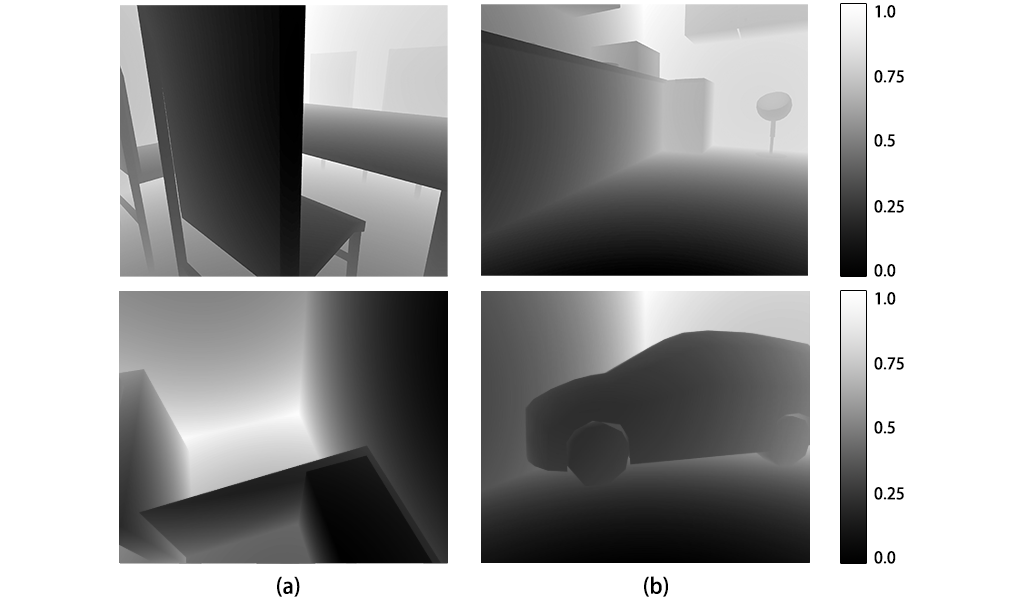
\includegraphics[scale=0.35]{img/depthmap/raw.png}
    \caption{\textbf{True depth map}}
    \label{fig:result_raw}
\end{figure}

We used Nvidia's synthetic data for initial training of our deep learning model. We captured 30 images from different positions of more than 900 different scenes with reflective objects placed in various positions in a room. The scenes were first rendered using transient rendering method[cite transient renderin paper] using same camera fov as kinect. The noise was then introduced to these scenes using FLAT's kinect sensor model. The model is trained on kinect data and hence understands the statistical properties of noise from the sensor. The model was then retrained on the data that we collected using a Canesta D350 3D Time-of-Flight camera. We collected 30 images each from 20 different scenes. All scenes had objects with varied specular properties, thus introducing MPI with varying amount. The ambient light was not controlled, providing very close to a real-world conditions.
%\lipsum[2-3]

% -----------------------------------------------------------------------
% Evaluation
% -----------------------------------------------------------------------

\section{Evaluation}

%\lipsum[2-3]
The first model is able to correctly predict the scene parameters to the accuracy of 66.4\%, when the noise (Base Error) present in the data is 0.022050m. The second model is able to predict a True Depth Map using the parameters from the first model as input.

We evaluated our model's output with respect to Nvidia's general pipeline for denoising 3D ToF camera data. We also performed evaluations against DeepToF and Phasor. We found that our model is able to perform better than Nvidia's Static Multi-Reflection Module (Static MRM). 

\begin{multicols}{4}
        \begin{figure*}[ht!]
            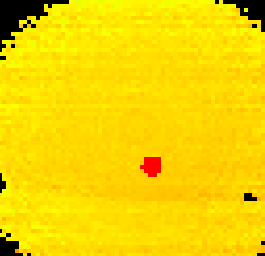
\includegraphics[width=.25\textwidth]{img/camera/1.png}\hfill
            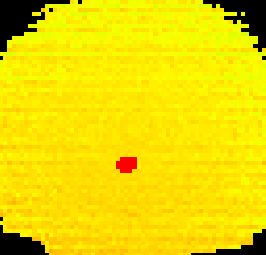
\includegraphics[width=.25\textwidth]{img/camera/2.png}\hfill
            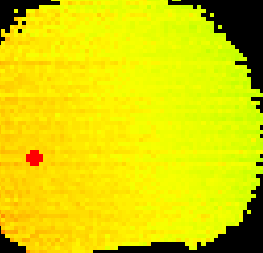
\includegraphics[width=.25\textwidth]{img/camera/3.png}\hfill
            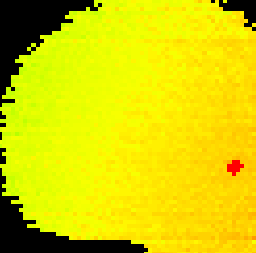
\includegraphics[width=.25\textwidth]{img/camera/4.png}\hfill   
            \caption{Raw measurements taken on a reflective whiteboard from different angles with Canesta DP205. The more red the closer. (left) centered slightly towards right. (mid-left) centered slightly towards left. (mid-right) towards left. (right) towards right. }
        \end{figure*}
\end{multicols}


% \begin{multicols}{3}
%         \begin{figure*}[ht!]
%             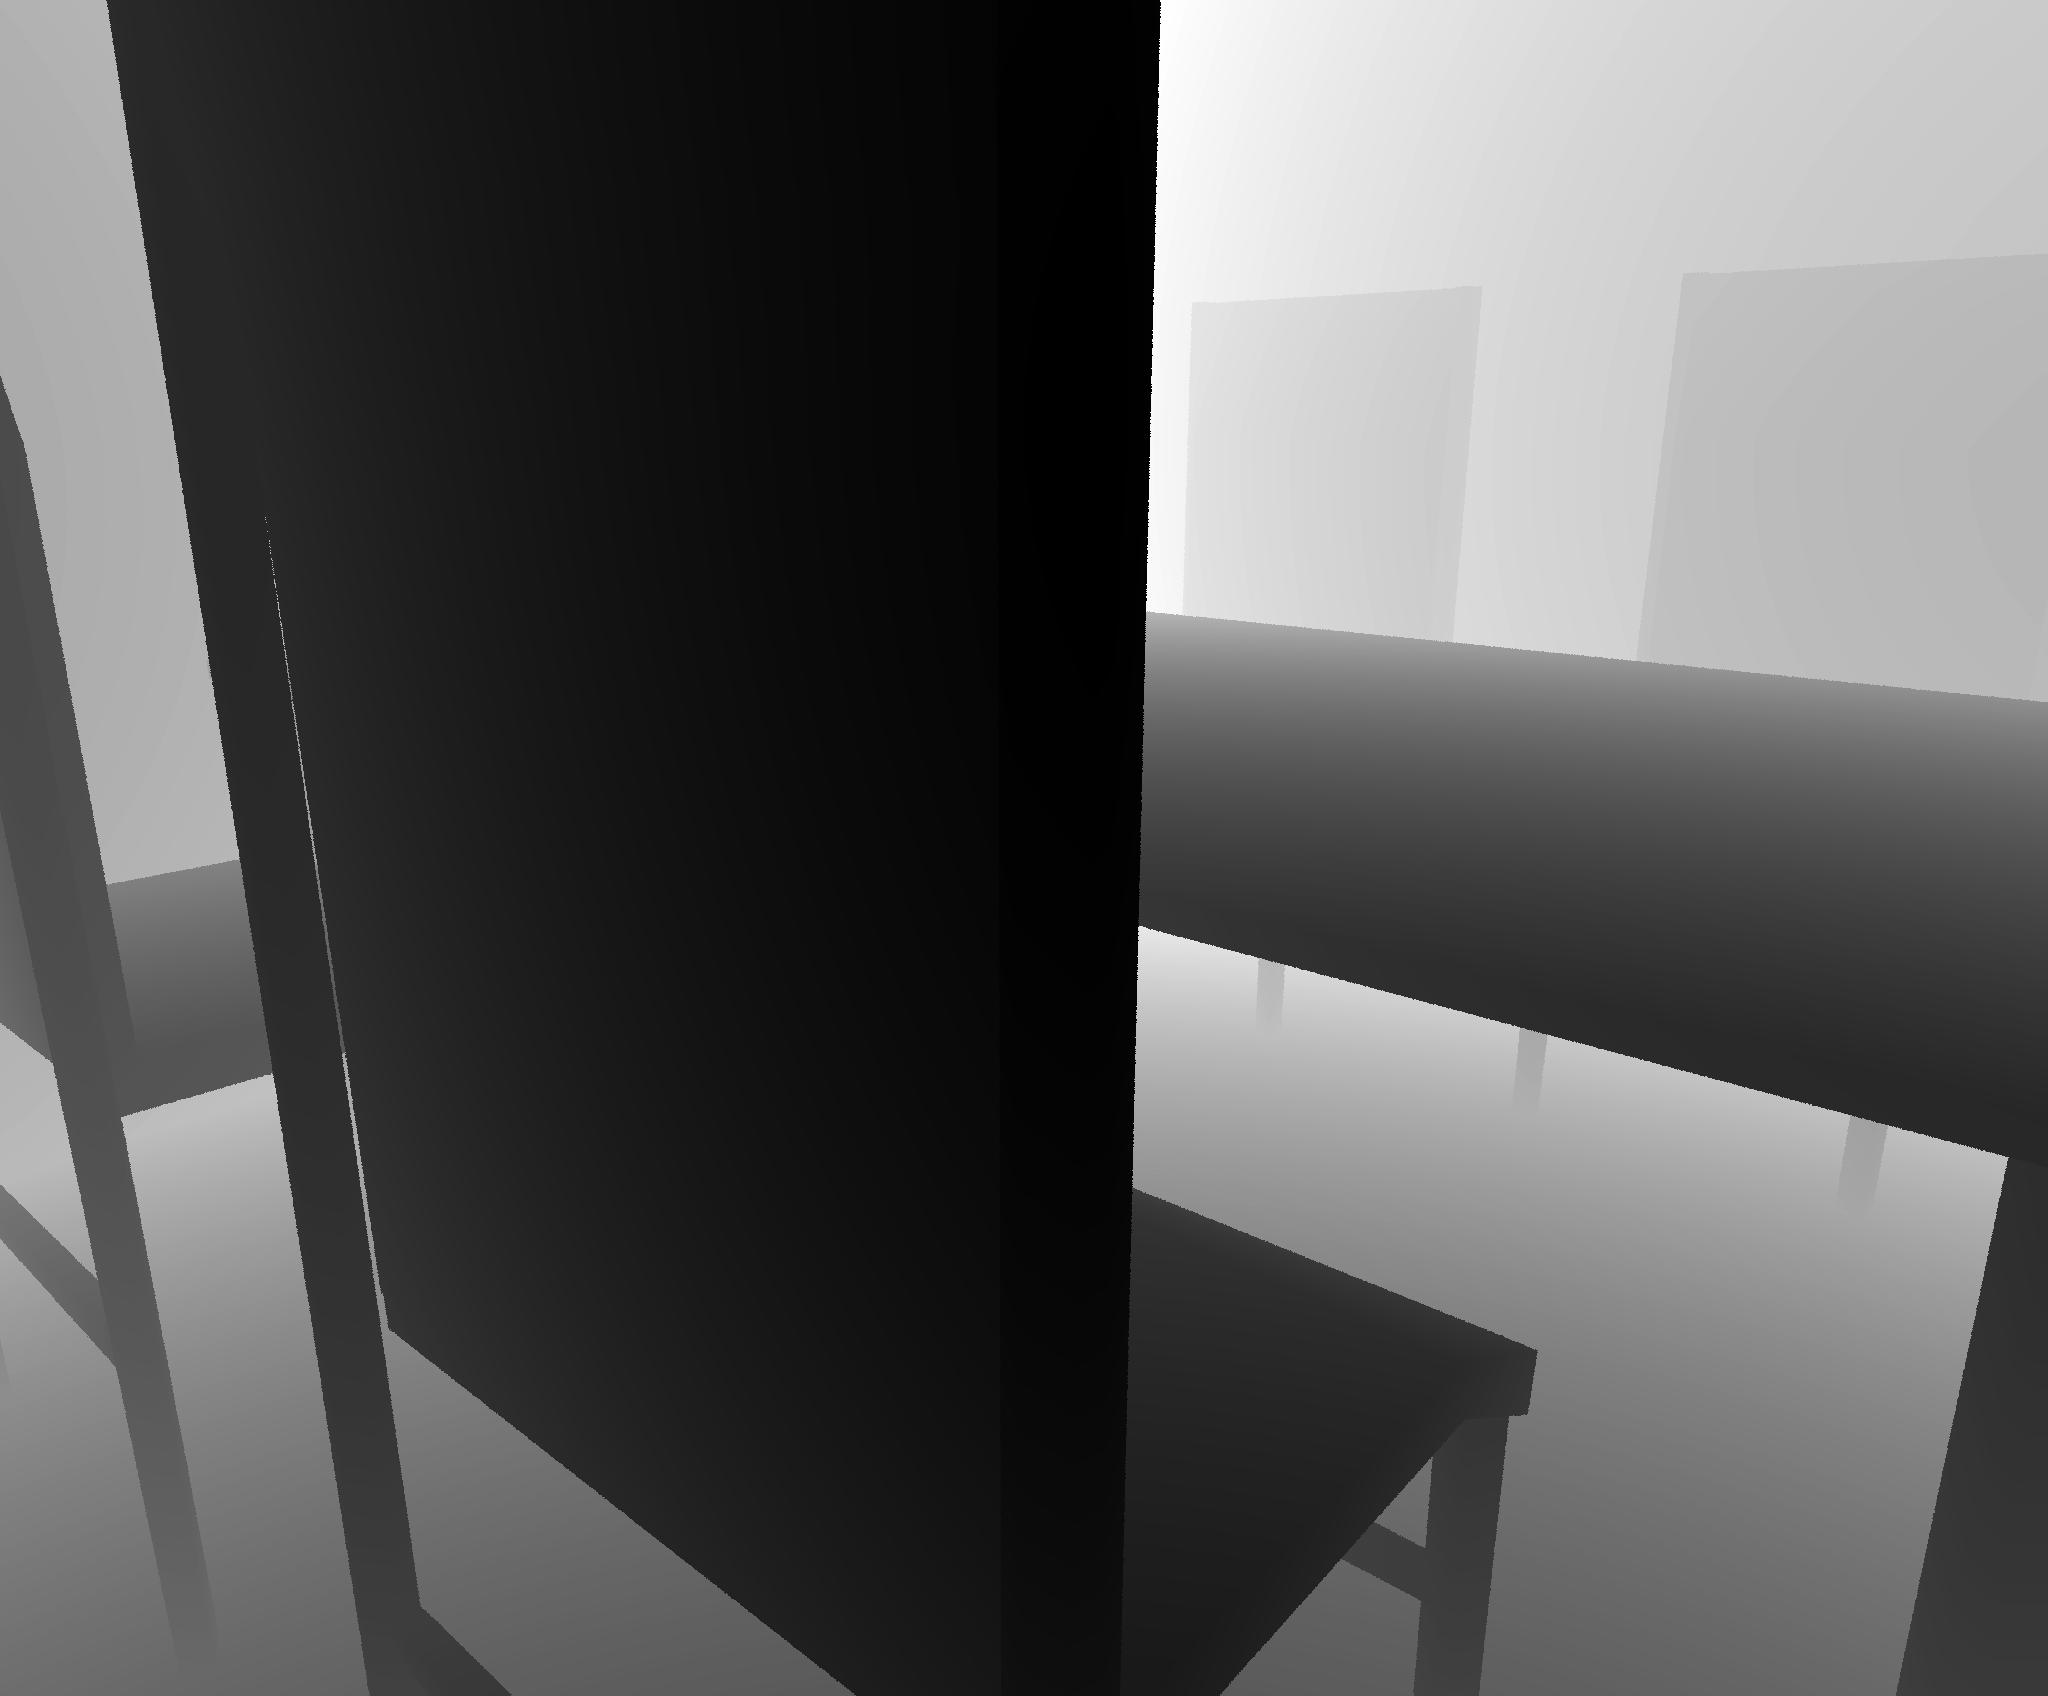
\includegraphics[width=.32\textwidth]{img/depthmap/1.jpg}\hfill
%             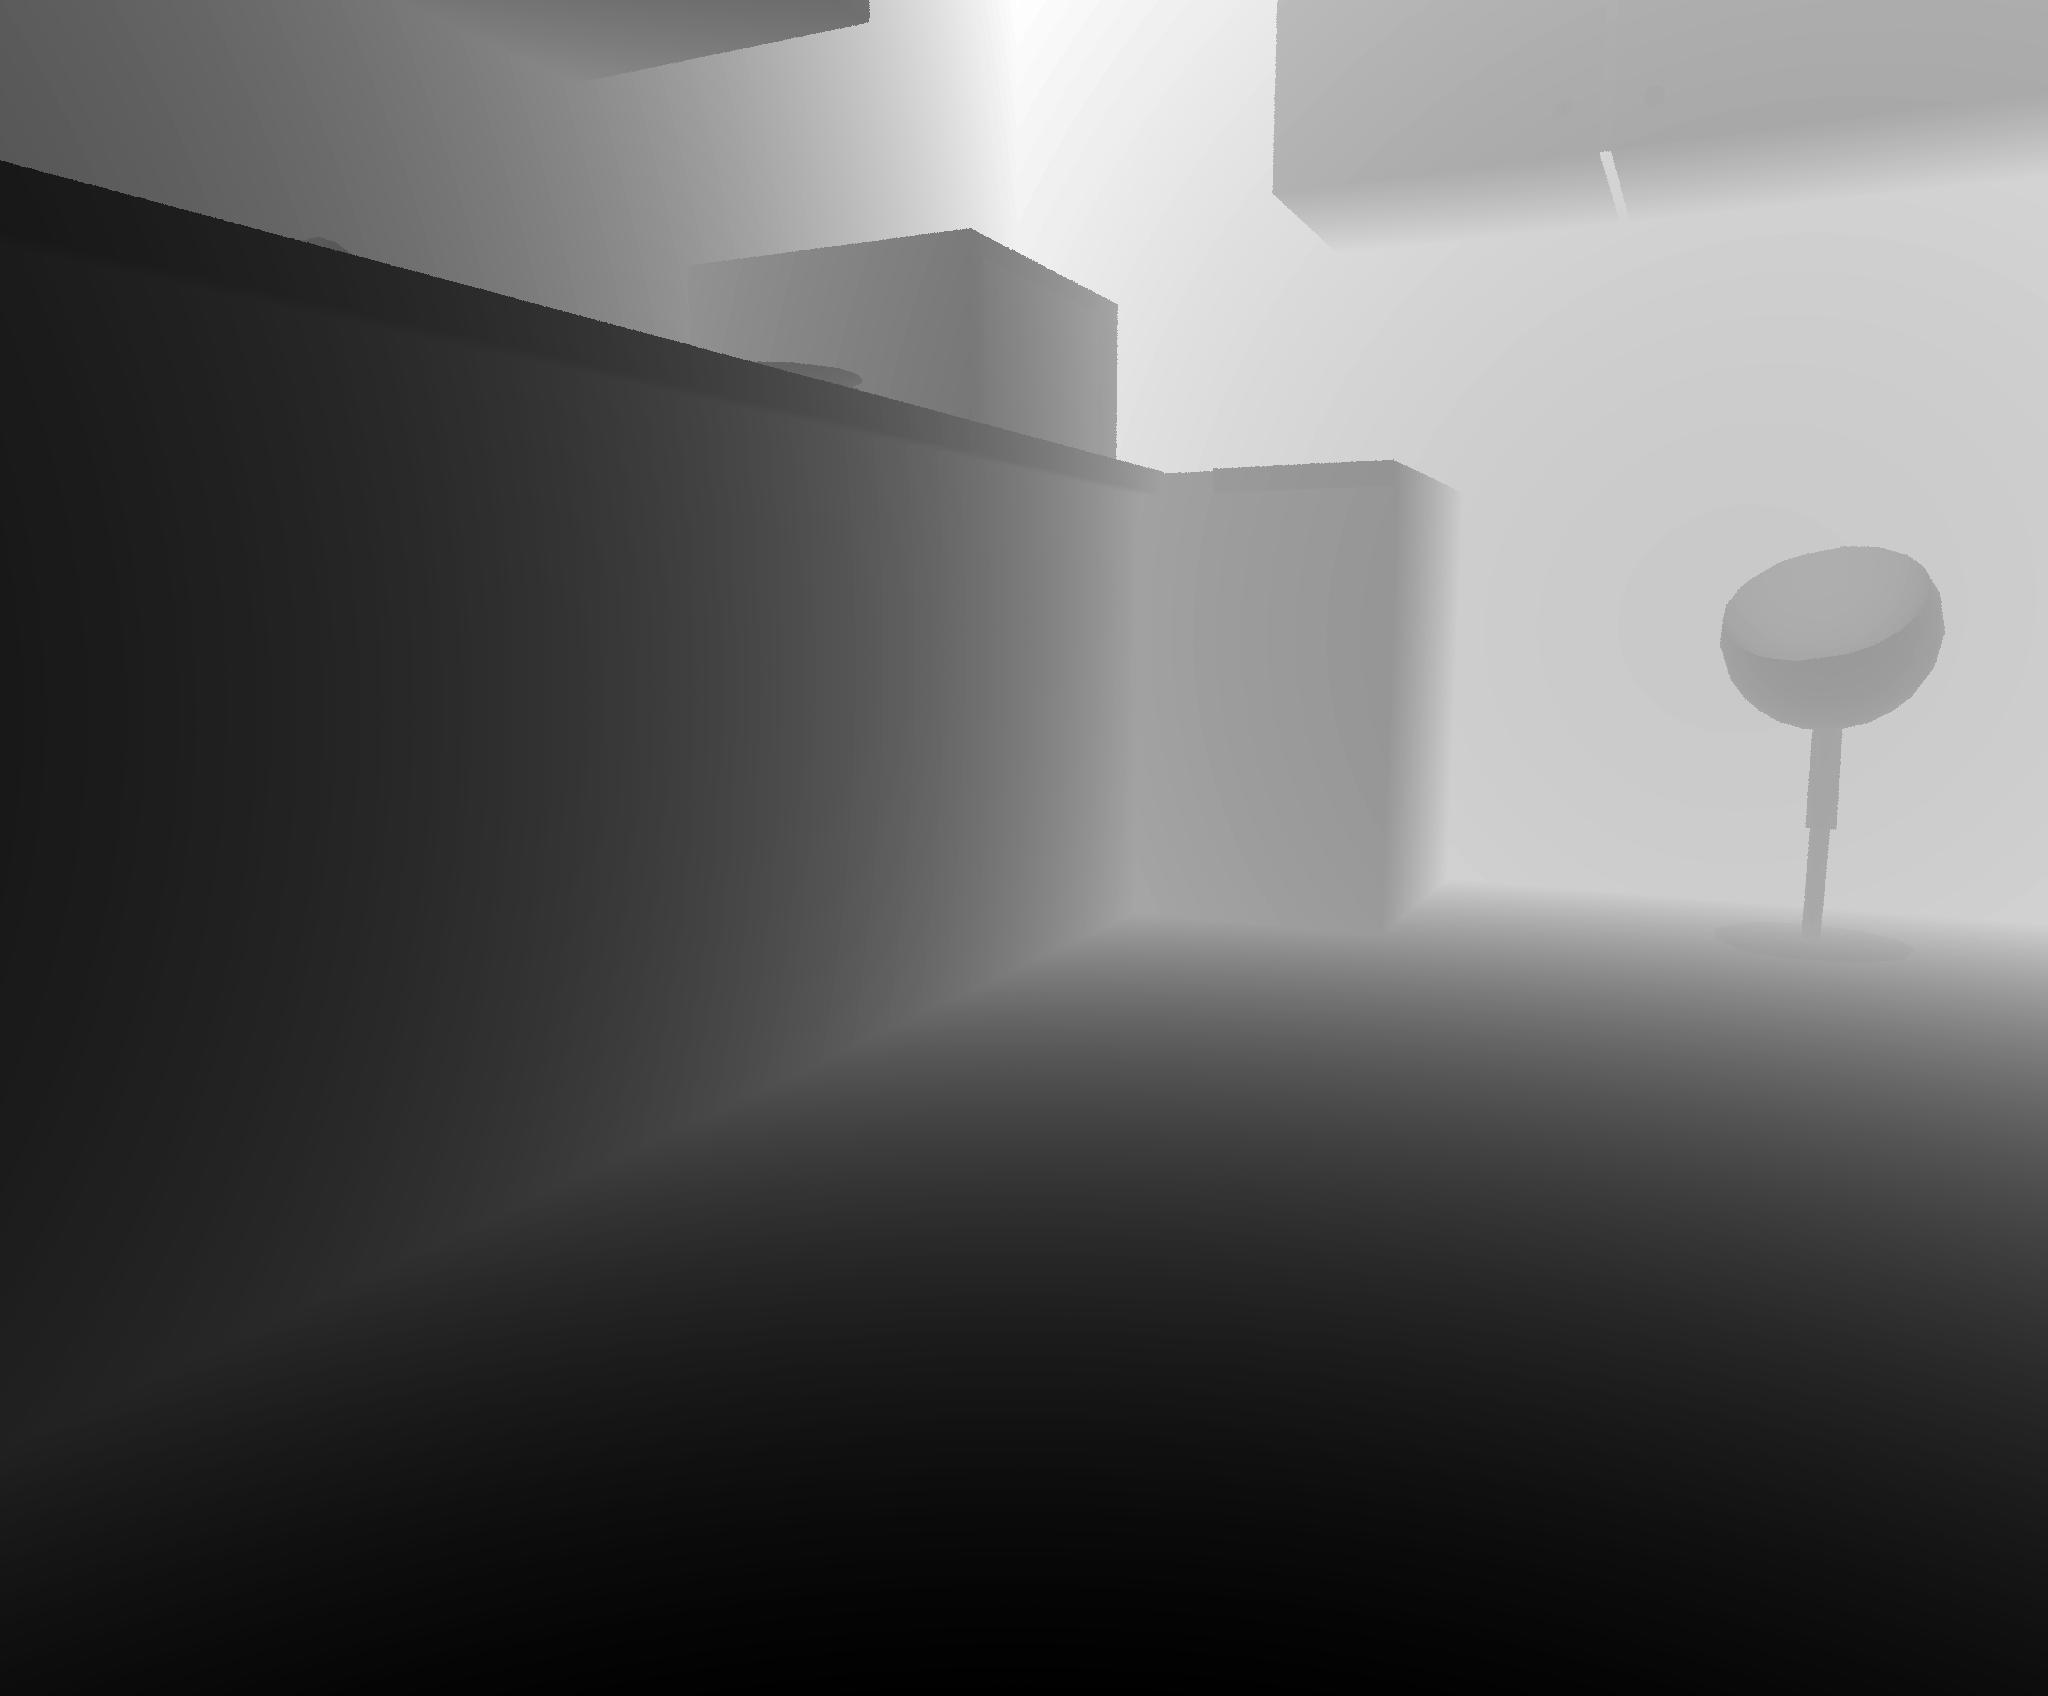
\includegraphics[width=.32\textwidth]{img/depthmap/2.jpg}\hfill
%             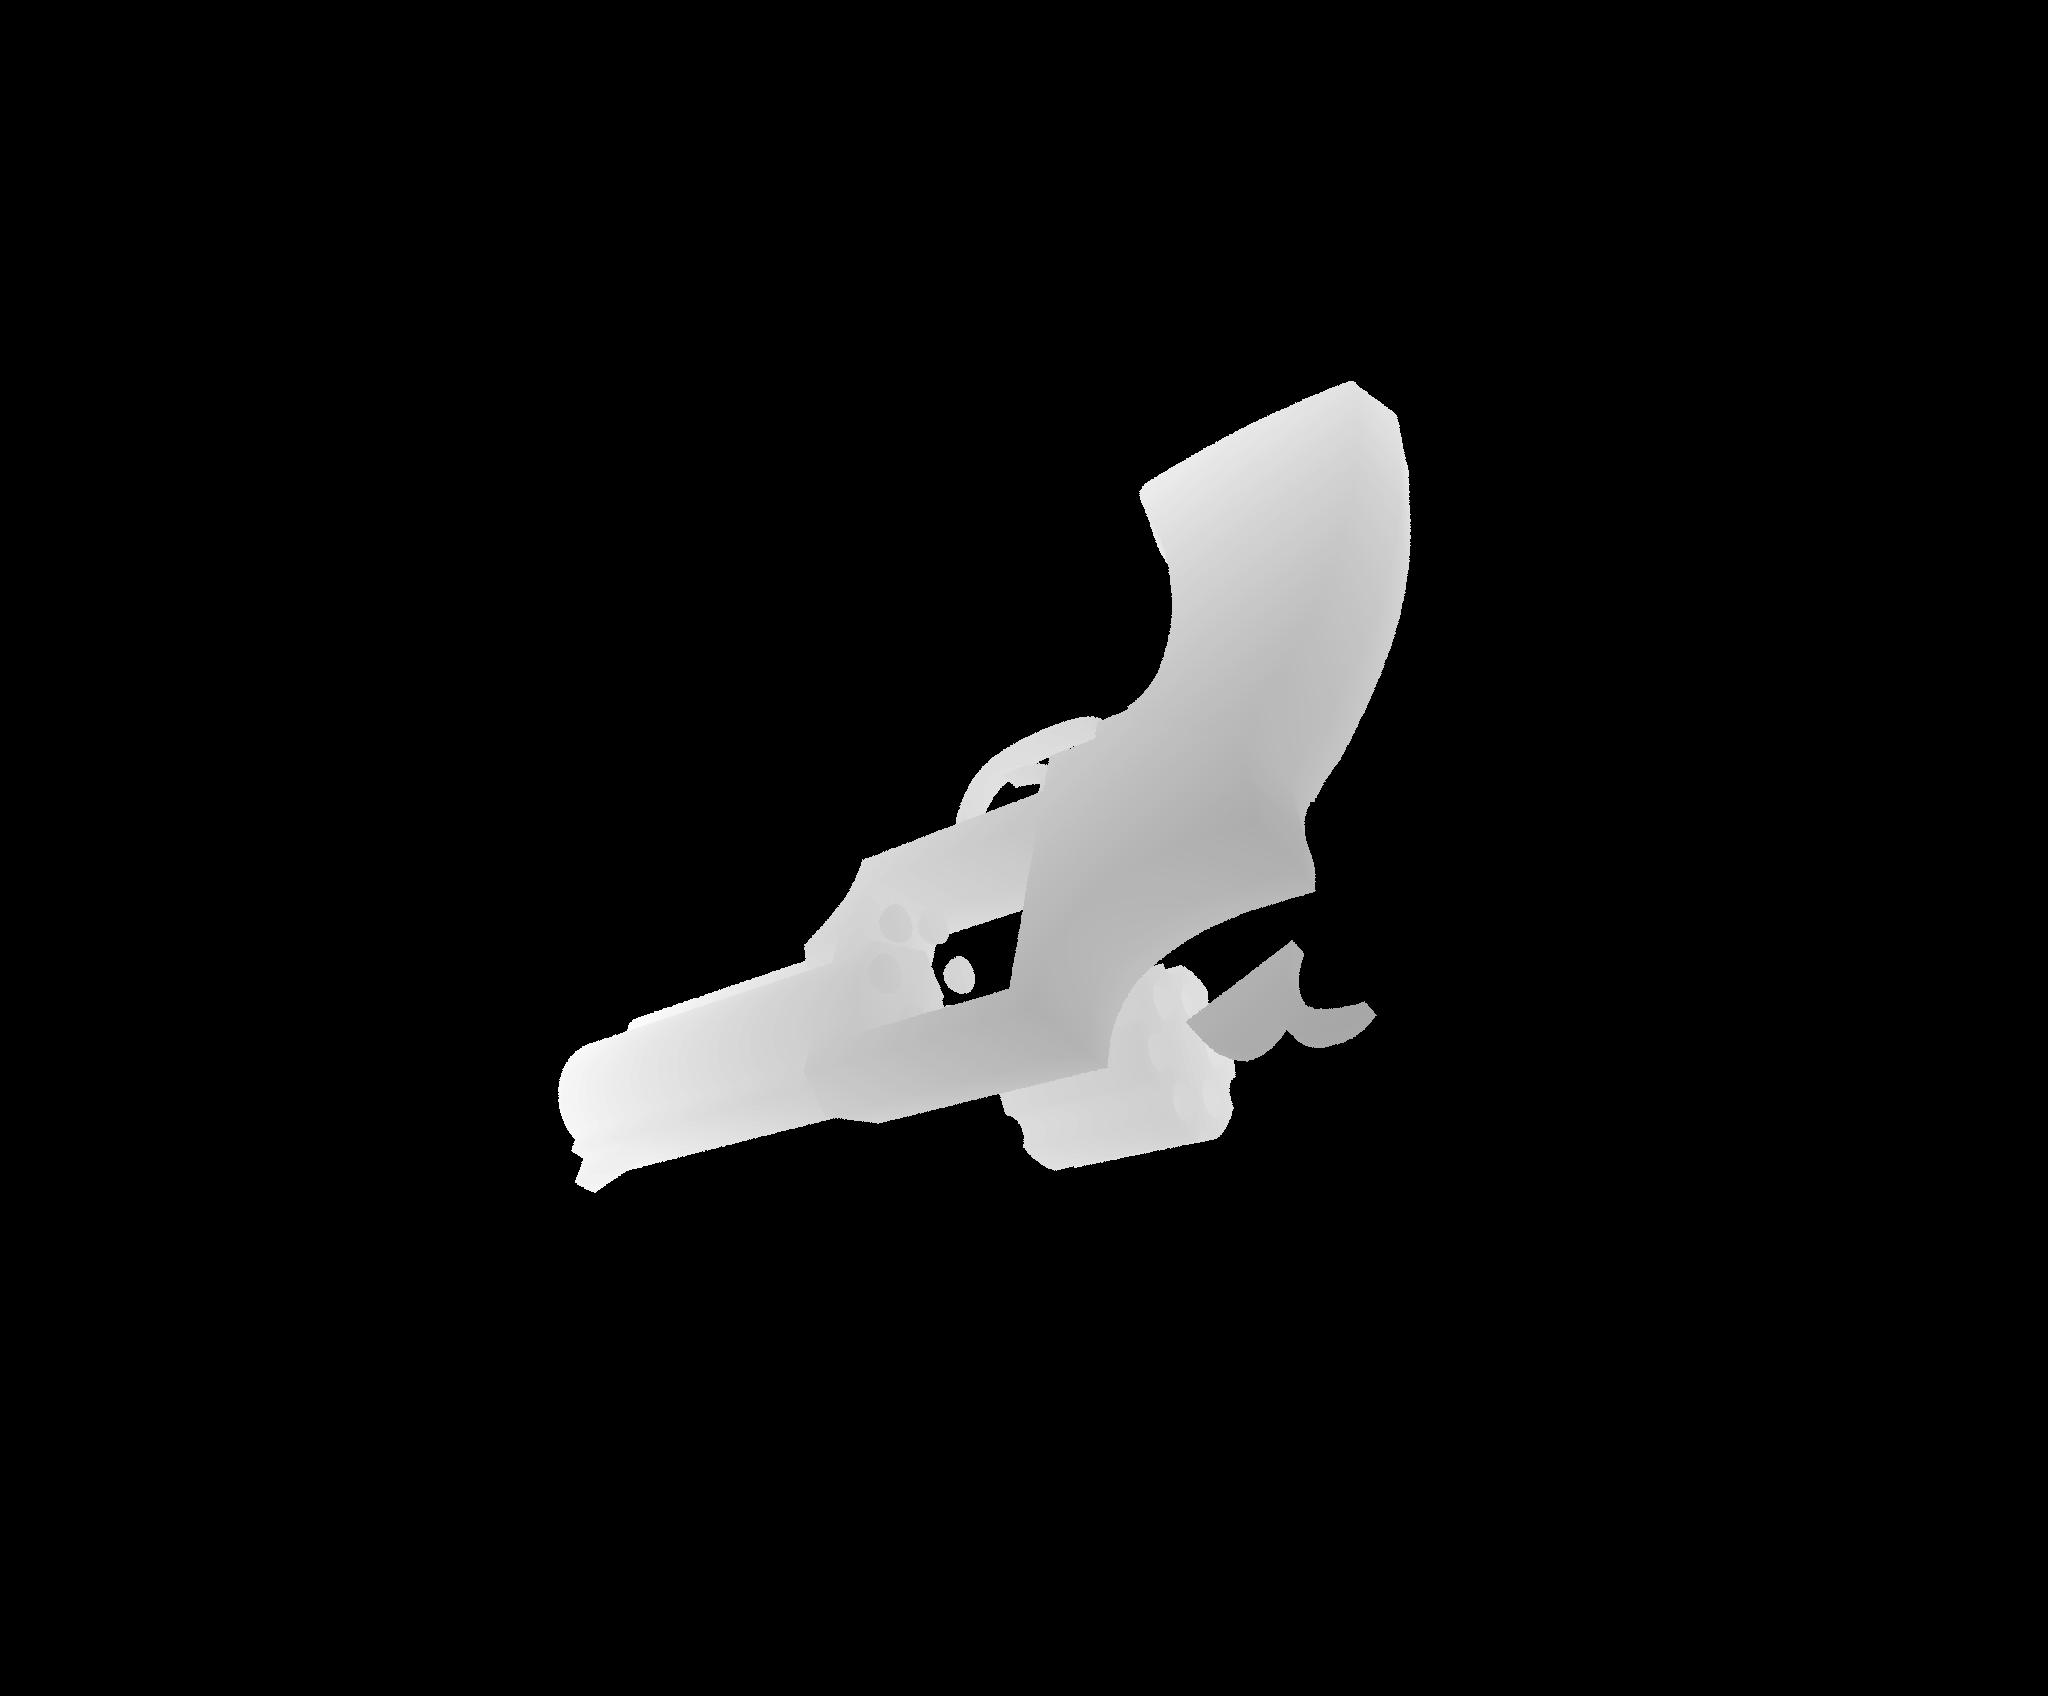
\includegraphics[width=.32\textwidth]{img/depthmap/3.jpg}\hfill   
%             \caption{ }
%         \end{figure*}
% \end{multicols}



% \begin{figure}
%     \centering
%     \includegraphics[scale=0.35]{img/result.png}
%     \caption{\textbf{Results of the proposed method on real-world data compared with synthesized data.}}
%     \label{fig:result_real}
% \end{figure}

\section{Limitations}
The model has been trained on synthetic dataset. The performance on real-dataset is not as good as seen in testing, because of difference in noise statistics between real data and data simulated using the NVidia FLAT simulator. 

We haven't included enough scenes with high specularity, and hence aren't able to handle objects present in a scene with high reflectance. 


% -----------------------------------------------------------------------
% Conclusion
% -----------------------------------------------------------------------

\section{Conclusion}

Multi-Path Interference based noise is difficult to eliminate because it is difficult to model all possible light paths in a complex scene. We have shown a deep learning technique that can be used to remove MPI based noise using two part deep learning network. 

%\lipsum[1]

% -----------------------------------------------------------------------
% Reference
% -----------------------------------------------------------------------

\bibliographystyle{abbrv}
\bibliography{ref}

\end{document}
